\subsubsection{Arquitectura del Sistema de Visión Artificial}

El sistema de visión artificial se estructura en tres módulos especializados que operan de manera coordinada durante los procesos de exploración y cosecha:

\textbf{Detector de Marcadores ArUco:} Identifica tubos de cultivo mediante marcadores visuales durante el escaneo vertical del workspace. Registra las posiciones verticales de todos los tubos detectados, generando un mapa que permite al sistema ubicar cada fila de cultivo.

\textbf{Detector de Cintas Verticales:} Localiza las cintas negras que sostienen las plantas individuales mediante análisis de contraste. Opera durante el escaneo horizontal de cada tubo para registrar las posiciones de todas las plantas presentes.

\textbf{Clasificador de Cultivos:} Determina el estado de madurez de cada planta mediante análisis morfológico de características extraídas de imágenes. Permite discriminar entre lechugas maduras listas para cosecha, plantas inmaduras, y posiciones vacías.

\begin{figure}[h]
\centering
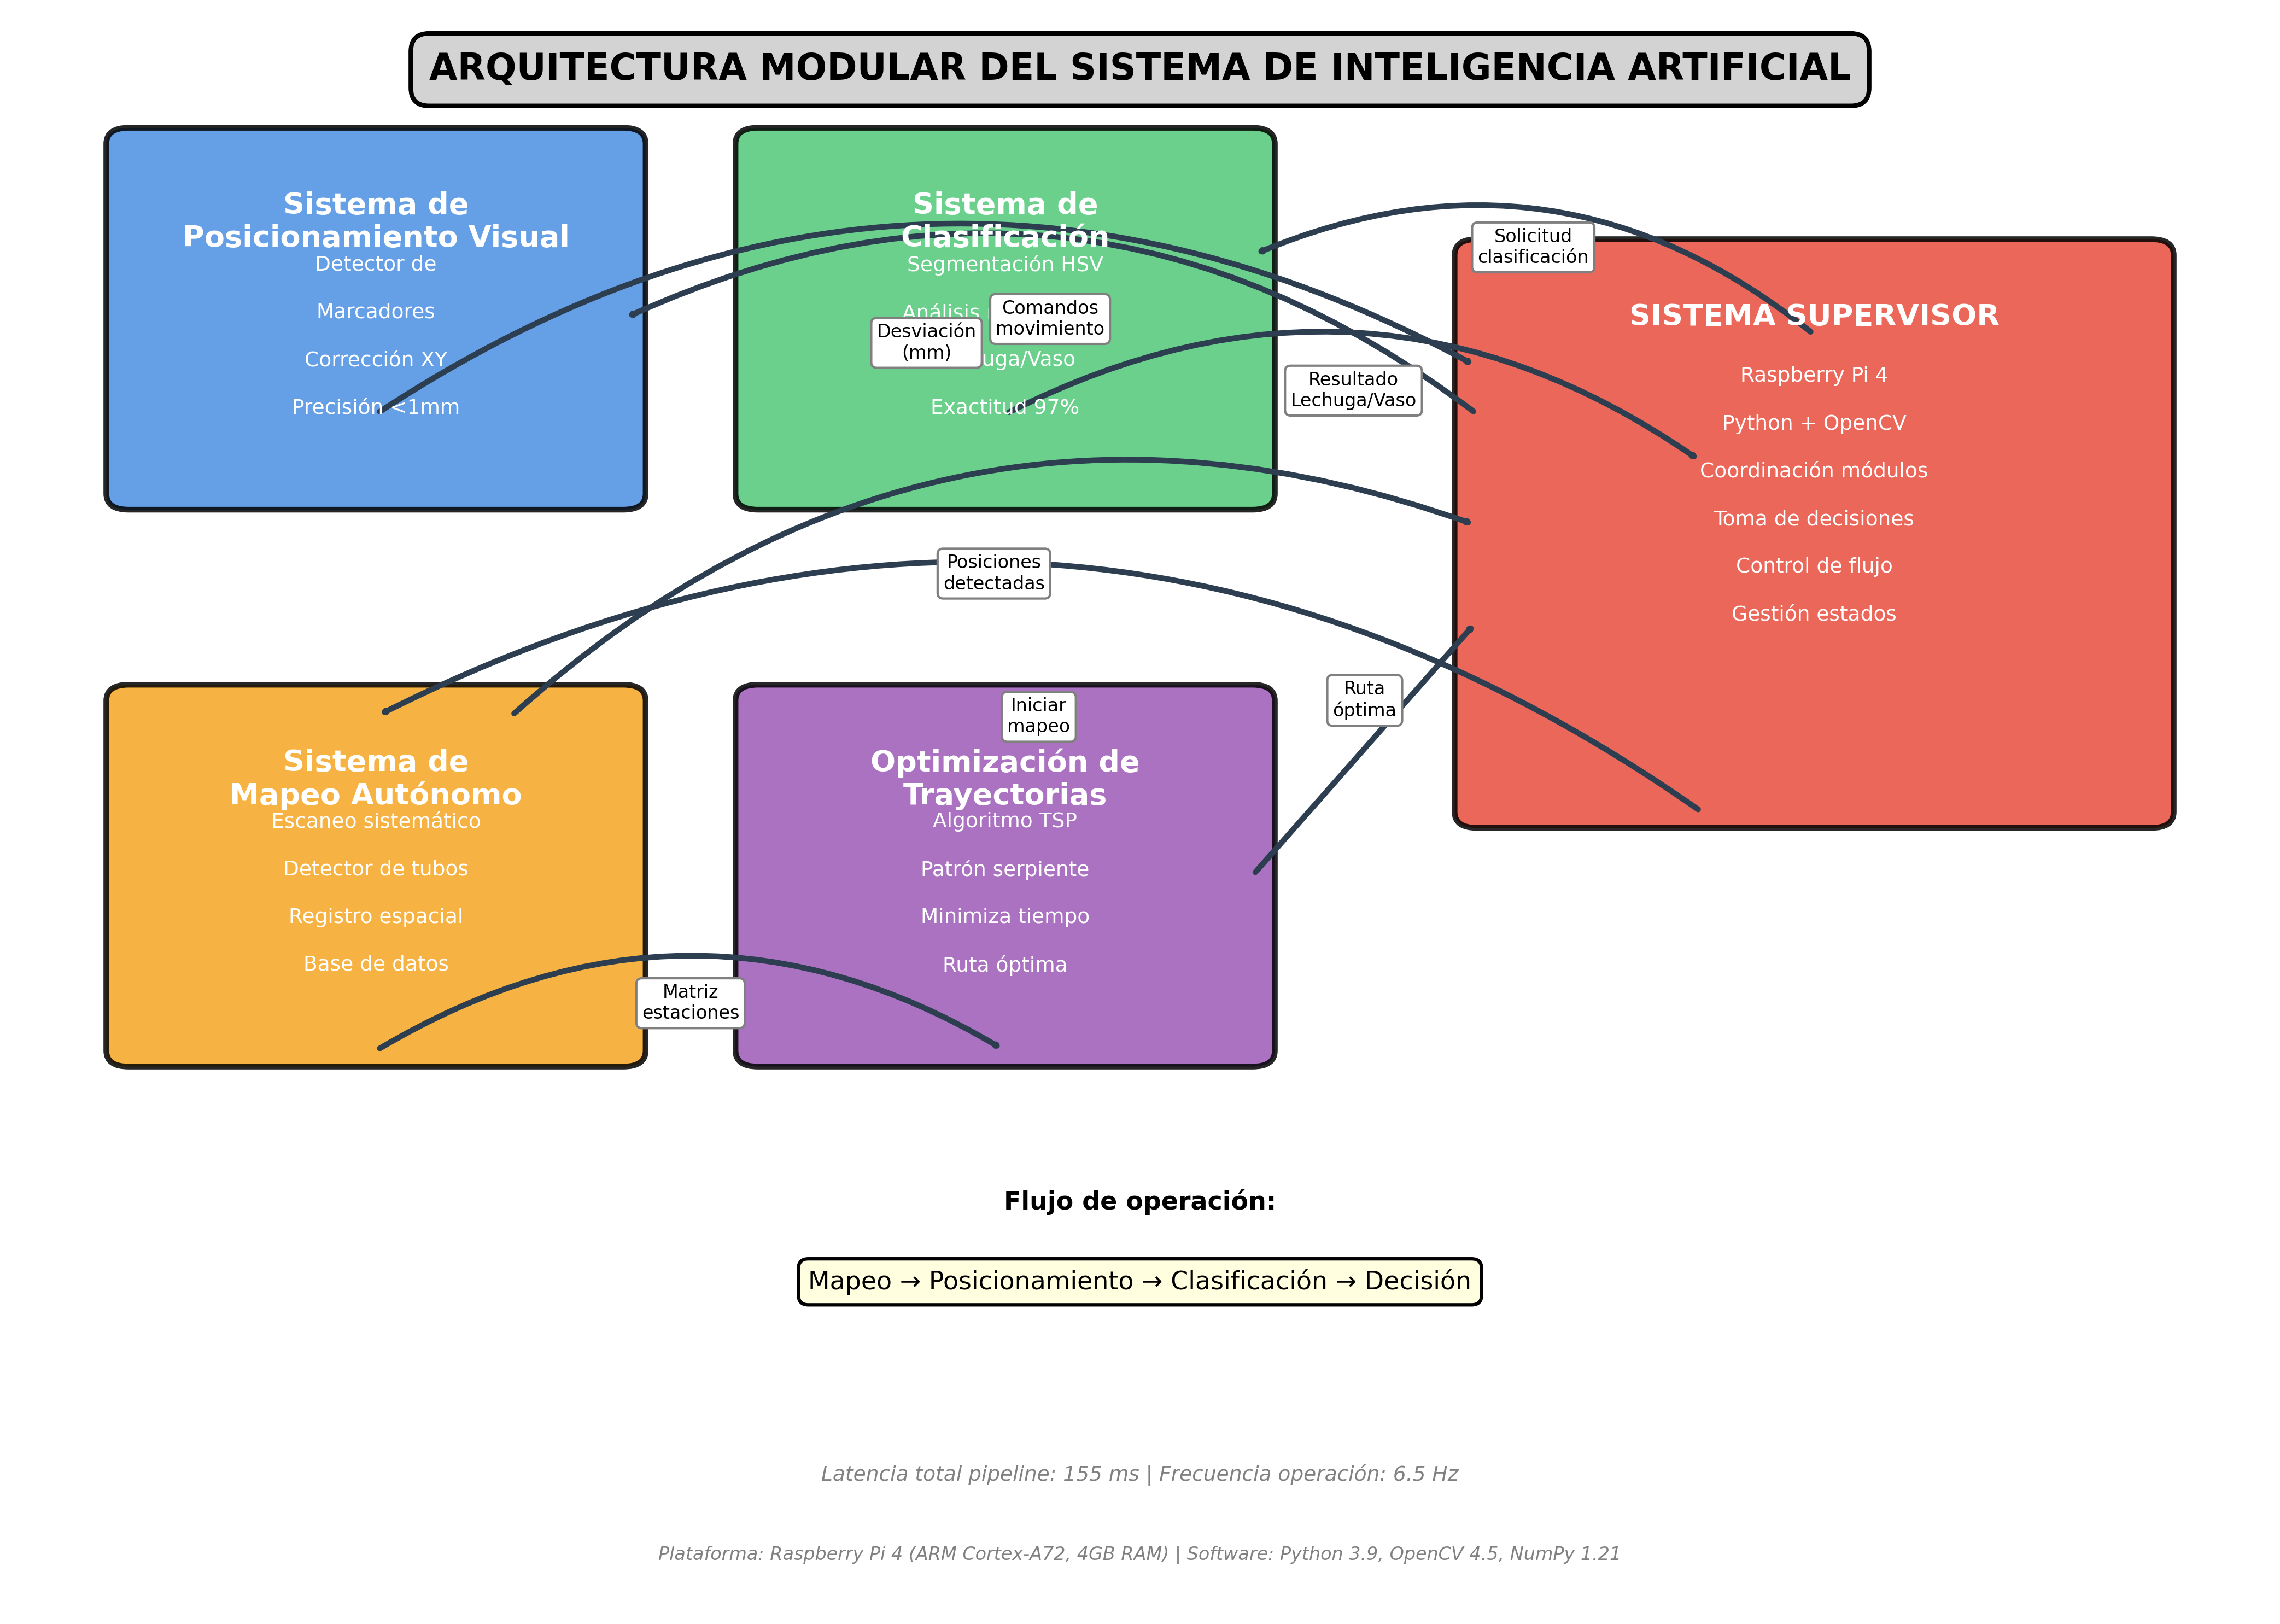
\includegraphics[width=0.85\textwidth]{imagenes/arquitectura_modular_ia.png}
\caption{Arquitectura modular del sistema de inteligencia artificial}
\label{fig:arquitectura_modular}
\end{figure}

El sistema se implementa sobre Raspberry Pi 5 con procesador ARM de cuatro núcleos y 8 GB de memoria RAM. Las bibliotecas empleadas incluyen OpenCV para procesamiento de imágenes, NumPy para operaciones matriciales, y PySerial para comunicación con el nivel regulatorio. El sistema operativo Raspberry Pi OS proporciona soporte nativo para los controladores de cámara.